\documentclass[12pt,a4paper]{article}
\usepackage[utf8]{inputenc}
\usepackage{geometry}
\usepackage{titlesec} % For customizing section titles
\usepackage{graphicx} % For images
\usepackage{hyperref} % For hyperlinks
\usepackage{fancyhdr} % For fancy headers and footers
\usepackage{lipsum} % For generating dummy text

% Set page geometry
\geometry{left=2.5cm, right=2.5cm, top=2.5cm, bottom=2.5cm}

% Set up hyperref
\hypersetup{
    colorlinks=true,
    linkcolor=black,
    filecolor=magenta,
    urlcolor=cyan,
}

% Customize section titles
\titleformat{\section}{\large\bfseries}{\thesection}{1em}{}
\titleformat{\subsection}{\normalsize\bfseries}{\thesubsection}{1em}{}

% Setup headers and footers
\pagestyle{fancy}
\fancyhf{}
\rhead{3D printing defect detection}
\lhead{AI Project Proposal}
\rfoot{Page \thepage}

% Title and author
\title{\textbf{AI Project Proposal 3D printing defect (spaghetti) detection }}
\author{Michal Raczkowski}
\date{10-01-2024}

\begin{document}

\maketitle
\thispagestyle{empty} % Remove header/footer for the first page

% Insert table of contents
\newpage
\tableofcontents
\newpage

\setcounter{page}{1} % Start page numbering from here

\section{Introduction}
\begin{itemize}
    \item \textbf{Focus:} Detecting 'spaghetti' defects in FFF 3D printing using AI image recognition.
    \item \textbf{Relevance:} Reducing material waste and improving safety in personal 3D printing.
\end{itemize}

\section{Domain Understanding}
\begin{itemize}
    \item \textbf{Problem:} 'Spaghetti' - Figure~\ref{fig:spaghetti3D}\ref{fig:spaghetti3D} defects due to print malfunctions or improper adjustments.
    \begin{figure}[h]
    \centering
    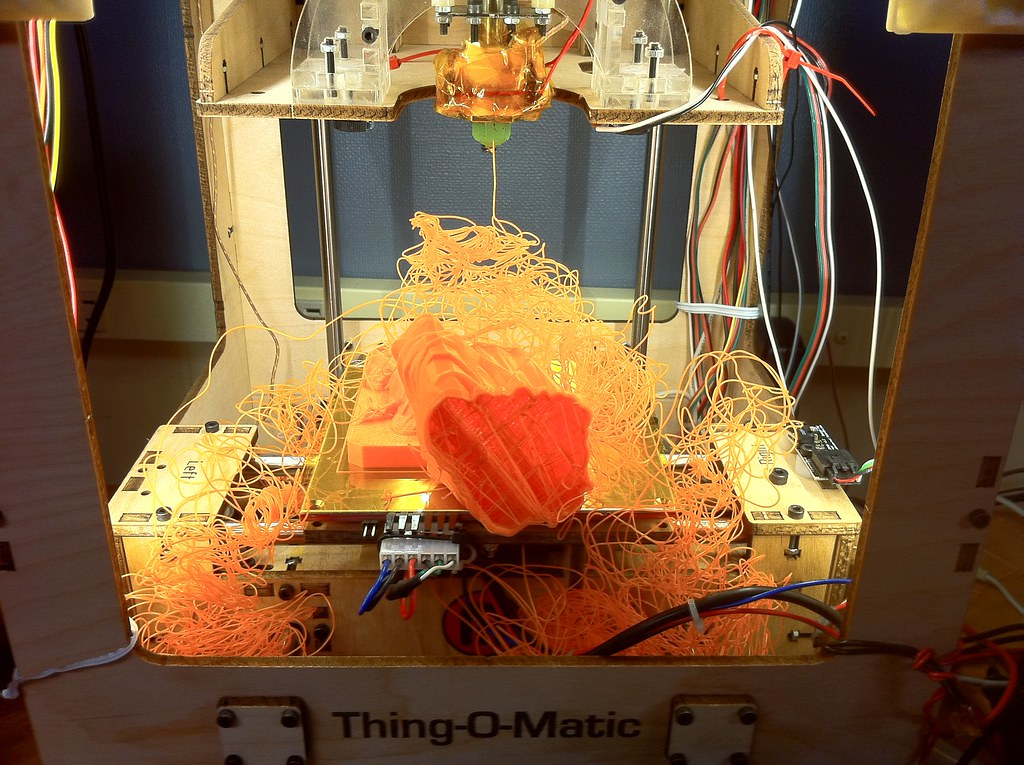
\includegraphics[width=0.5\linewidth]{spaghetti3D.jpg}
    \caption{Extruded filament that resembles spaghetti}
    \label{fig:spaghetti3D}
    \end{figure}

    \item \textbf{Research:} Focused on understanding the 3D printing process and defect characteristics.
\end{itemize}

\section{Data Sourcing}
\begin{itemize}
    \item \textbf{Data Type:} Images (.jpeg, .png) of 3D prints, both defective and non-defective.
    \item \textbf{Collection:} Homemade pictures and open-source online repositories.
\end{itemize}

\section{Analytic Approach}
\begin{itemize}
    \item \textbf{Objective:} Identify 'spaghetti' defects in 3D printed models.
    \item \textbf{Target Variable:} 'Defect Status' (0 for absent, 1 for present).
\end{itemize}

\section{Data Preparation}
\begin{itemize}
    \item \textbf{Process:} Standardize image size/format, normalize pixel values, annotate, and label.
\end{itemize}

\section{Modeling}
\begin{itemize}
    \item \textbf{Approach:} Use YOLO variants for defect detection.
    \item \textbf{Metrics:} IoU, AP, mAP, Precision, Recall, F1 Score.
\end{itemize}

\section{Conclusion}
\begin{itemize}
    \item \textbf{Impact:} Enhancing quality control in 3D printing, reducing waste and risks.
\end{itemize}

\end{document}
